\section{Recognition Strategies}
\label{sec:background:recognition_strategies}

The \gls{icdar} Robust Reading Competitions \citep{Lucas:2003iw, Lucas:2005bq, Shahab:2011hq, Karatzas:2013by, Karatzas:2015tj} broke down the issue of text extraction into two sub-problems: text locating and character recognition. Most of the literature discussed in Section~\ref{sec:background:detection_strategies} focused within the text locating sub-problem. For character recogntion, the \textit{Focused Scene Text} word recognition task\footnote{See Challenge 2, Task 3 in \citep{Shahab:2011hq, Karatzas:2013by}.} received three entries in 2011 and four in 2013. In 2015, the recognition challenge was redesigned\footnote{See Challenge 4, Task 3 in \citep{Karatzas:2015tj}.} using a new (and more challenging) \textit{Incidental Scene Text} dataset of photos captured in-the-wild using Google Glass. The evaluation scheme uses the \textit{Total Edit Distance} metric (described in \citep{Karatzas:2013by}) and additionally the number of correctly recognised words for qualitative analysis. Table~\ref{tab:background:recognition_strategies:icdar_results} summarises the top-scoring recognition rates from these competitions.

\begin{table}[bh]
  \centering
  \caption{Top-scoring word recognition results from ICDAR 2011--2015.}
  \label{tab:background:recognition_strategies:icdar_results}
  \tablefit{
    \begin{tabular}{lll|cc}
      \toprule
        \textbf{Year} &
        \textbf{Method} &
        \textbf{Dataset} &
        \textbf{Total Edit Distance} &
        \textbf{Correctly Recognised Words (\%)}
      \\
      \midrule
        2011 &
        TH-OCR System \citep{Liu:2005uw} &
        Focused &
        176.23 &
        41.2
      \\
        2013 &
        PhotoOCR \citep{Bissacco:2013vj} &
        Focused &
        122.7 &
        82.83
      \\
        2015 &
        MAPS \citep{Kumar:2012kh} &
        Incidental &
        1128.0 &
        32.93
      \\
      \bottomrule
    \end{tabular}
  }
\end{table}

It has been widely demonstrated that off-the-shelf commercial and open source OCR packages are able to correctly recognise text once the characters are extracted. In their conclusions of the ICDAR 2015 competition, \citeauthor{Karatzas:2015tj} note that the top performing methods will make use of commercial \glspl{ocr} and conclude that conventional shape-based \gls{ocr} engines can produce competitive results with pre-processed images. 

This conclusion is emphasised in further works. The Open Source Tesseract \gls{ocr} engine was used in \citet{Benami:2012jf} to extract \glspl{rbn} after preprocessed \gls{cc}-based extraction. Similarly, leading commercial \gls{ocr} engines used by \citet{XiangrongChen:2004ha} were able to achieve 93\% recognition from binarised text regions after AdaBoost non-text classification, using ABBYY FineReader\footnoteurl{https://www.abbyy.com}{3 July 2017}, TOCR\footnoteurl{http://www.transym.com}{3 July 2017} and Readiris Pro\footnoteurl{http://www.irislink.com/readiris}{3 July 2017}. Similarly, \citet{Gatos:2005wd} used ABBYY FineReader and showed their extraction method showed a 50\% improvement for indoor and outdoor scene images, an approach also applied by \citet{XiangrongChen:2004ha}. This is not to say that \gls{ocr} engines are always needed.

Recent interest in developing novel general character recognition strategies have also been investigated. \citet{Wang:2011tw} compared ABBYY FineReader with their novel PLEX approach and demonstrated that their text recognition system can outperform traditional \gls{ocr} engines without the use of a text detector. This inspired more recent works: in \citeyear{Lee:2016uy}, \citet{Lee:2016uy} developed a lexicon-free photo \gls{ocr} frameworks. Furthermore, application-specific recognition has been investigated using variant techniques.

\begin{figure}[h]
  \centering
  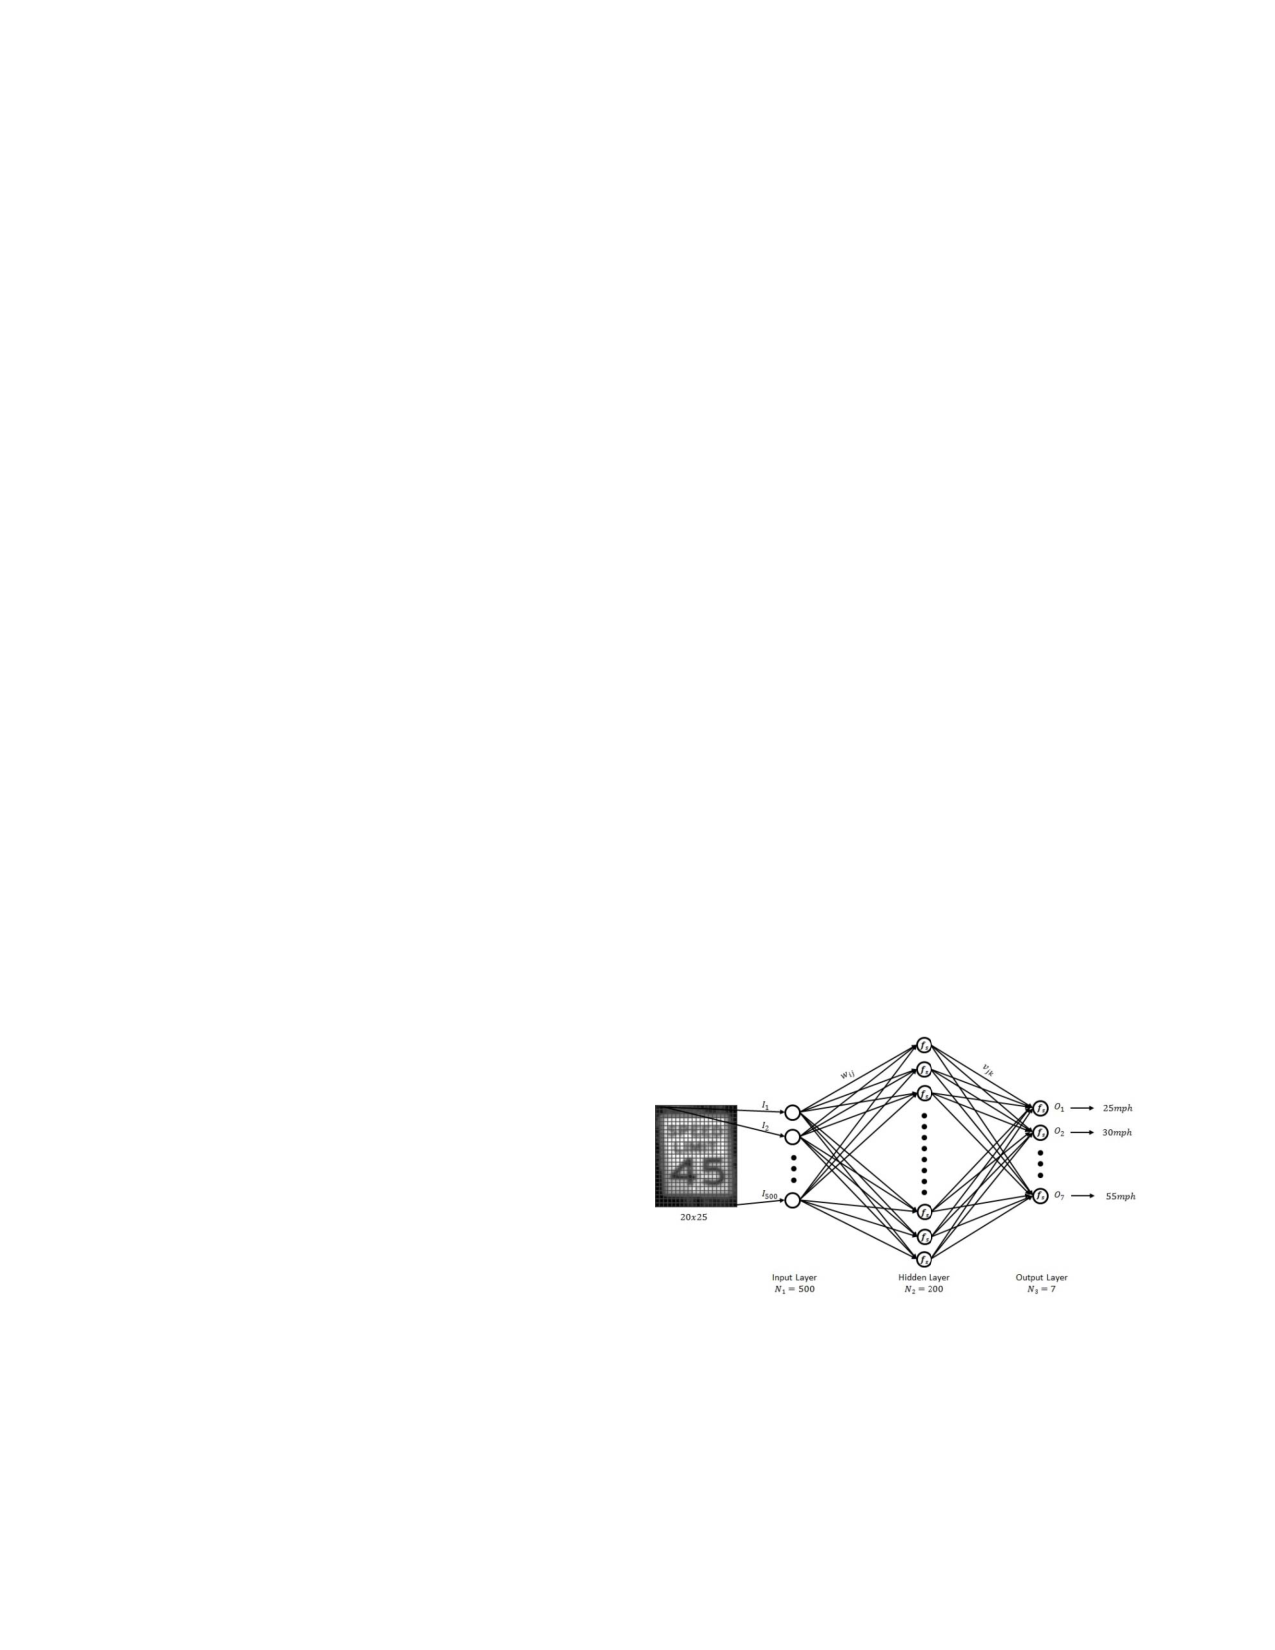
\includegraphics[width=0.75\textwidth]{images/background/kundu2015_nn}
  \caption[A NN designed to recognised speed limit signs]{The artificial \glsx{mlp} \gls{nn} designed in \citet{Kundu:2015vq} to recognise US-style speed limit signs.}
  \label{fig:background:recognition:kundu2015_nn}
\end{figure}

A \citeyear{Kundu:2015vq} study into \glsplx{tsr} to detect US-style speed limit signs achieved recognition without the use of any OCR packages. In \citep{Kundu:2015vq}, \citeauthor{Kundu:2015vq} were able to extract a speed limit sign via the use of \glspl{mser} and template matching. The resulting detected signs were scaled to a grayscaled size of $20 \times 25$ pixels and fed into a \glsx{mlp} \gls{nn} of 200 neurons in the hidden layer. The output layer of the network consisted of seven nodes, each representing the seven kinds of speed limit signs in US cities (25, 30, 35, 40, 45, 50, and 55 miles per hour). This architecture is shown in Figure~\ref{fig:background:recognition:kundu2015_nn}. When trained with 13,289 images of text cases and 4,319 non-text cases, the results showed that their recognition classier was able to correctly recognise speed limit signs with an accuracy of 98.04\%. Similar results were achieved using a feed-forward \gls{mlp} in \cite{Eichner:2008dw}, using UK/Poland style speed limits scaled to $20 \times 20$ pixels (grayscale) and 12 output layer neurons ($10 \dots 100$ kilometres per hour, the national speed limit sign, and non-sign neurons).

However, works in \gls{tsr} systems that utilise networks are generally non-generalisable, and only work in a limited context (i.e., by classifying speed limit signs of known outputs). In our context of \gls{rbn} recognition, we have a known character output range of 36 possibilities: 0--9 and A--Z = 10 + 26. We do not consider lowercase letters.

Beyond \gls{tsr} systems, however, we see the use of more generalisable networks: \citet{Netzer:2011to} trained neural network to recognise street number characters from Google Street View with higher precision and recall than that of \gls{hog} and the Tesseract \gls{ocr} engine, showing that the applicability of \glspl{nn} for recognition can outperform traditional means. \citet{Anagnostopoulos:2006wv} used a \gls{pnn} to recognise single characters of the same 36 possibility range (i.e., uppercase alphanumeric characters) corresponding to the input grayscale vector of $9 \times 12$ pixels ($9 \times 12 = 108$ input neurons) for a single character. Figure~\ref{fig:background:recognition:anagnostopoulos2006_nn} illustrates the \gls{pnn} architecture used in this study. Furthermore, investigations in comparing different architectures of \glspl{nn} for this context is given in \citet{Lee:2016uy}.

\begin{figure}[h]
  \centering
  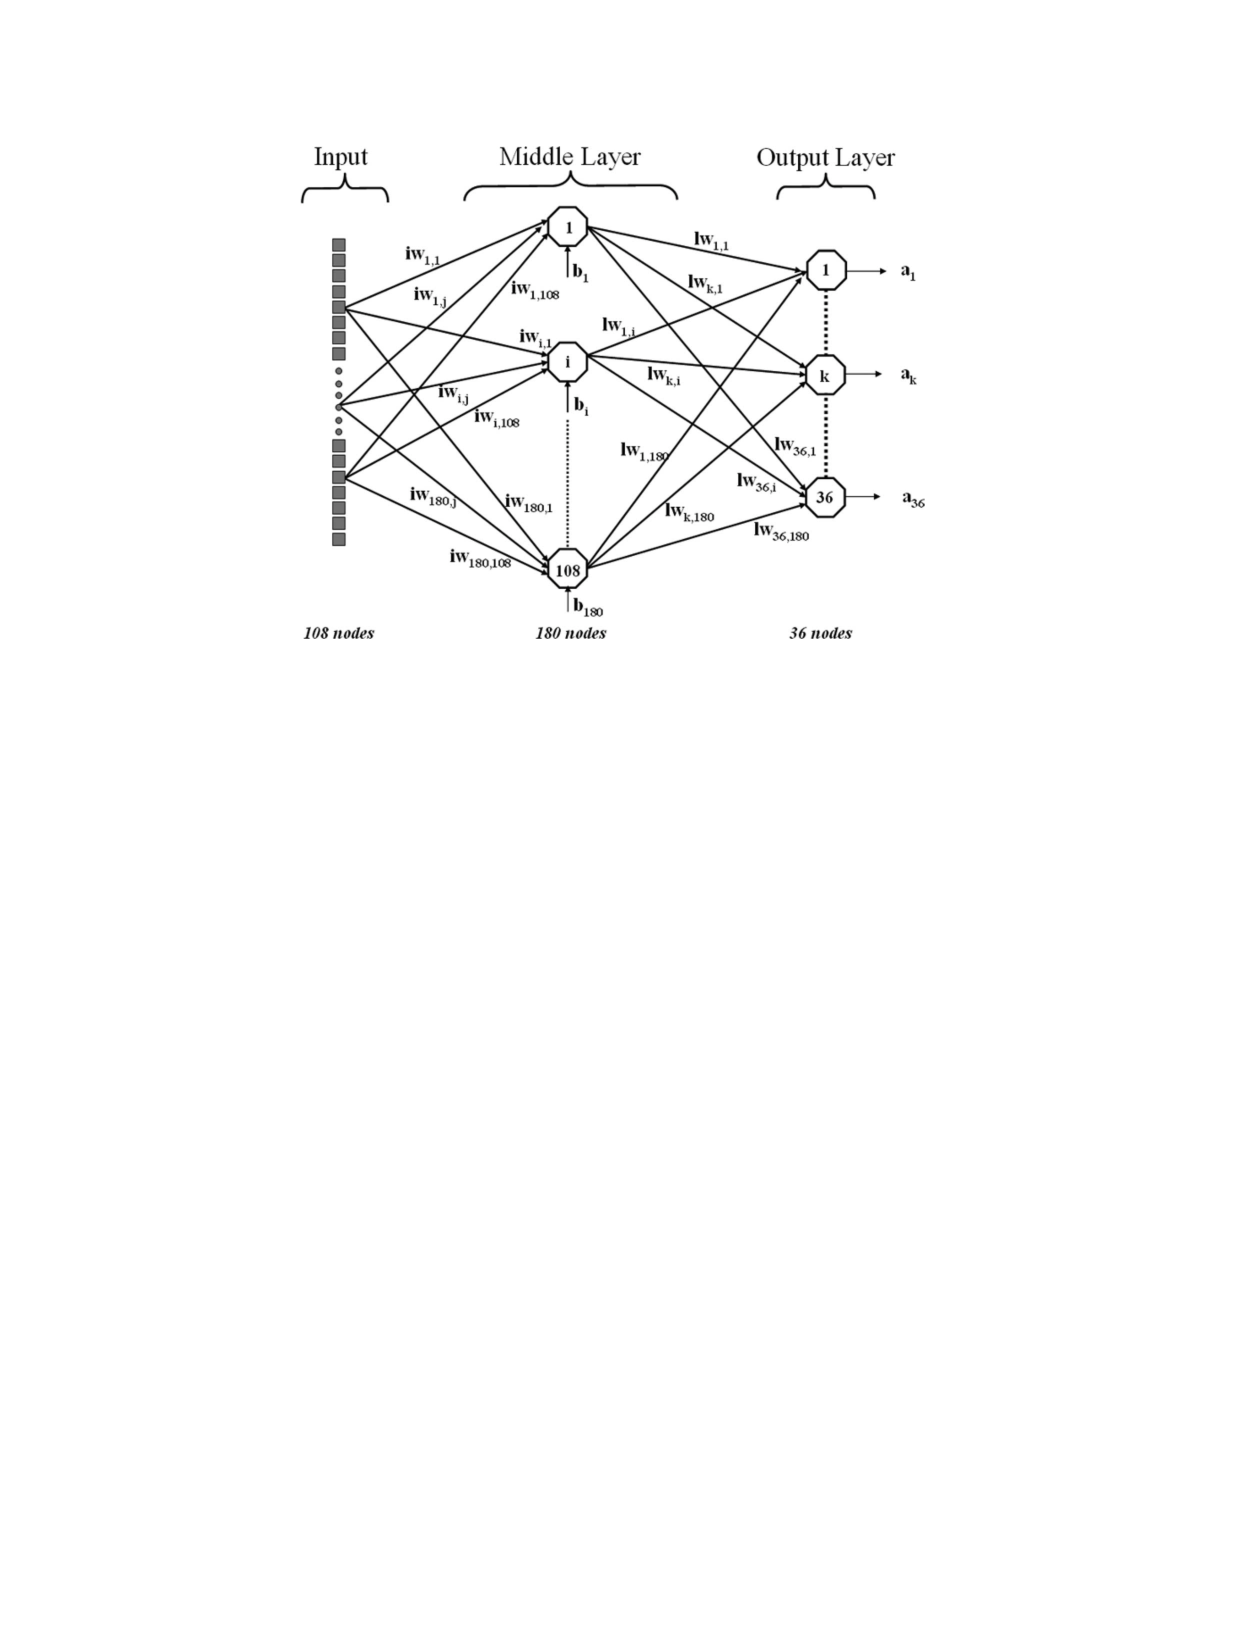
\includegraphics[width=0.75\textwidth]{images/background/anagnostopoulos2006_nn}
  \caption[A PNN used to recognise license plate characters]{\citet{Anagnostopoulos:2006wv} developed the architecture of a \gls{pnn} to determine a single character from within a license plate.}
  \label{fig:background:recognition:anagnostopoulos2006_nn}
\end{figure}


However, these pipelines are still entirely dependent on good detection strategies, and in the case where classifiers are used, quality training data must be supplied. The pipeline developed by \citet{Benami:2012jf} for \gls{rbn} detection (Figure~\ref{fig:background:recognition:benami2012_pipeline}) is dependent on quality facial detection: the OpenCV implementation \citep{Lienhart:2002uo} was used in this study. In order to detect the torso region---and thus detect the bib sheet itself---a heuristically-driven calculation is used to hypothesise where the torso bounds ($T_{b} = T_{h} \times T_{w}$) are, given by the face height ($F_{h}$), face width ($F_{w}$):
\begin{equation*}
  T_{b} = (3 \times F_{h}) \times (\frac{7}{3} F_{w})
\end{equation*}
The location of $T_{b}$ is horizontally located at the centre of the face midpoint and vertically halfway below the face height ($0.5 \times F_{w}$). Hence, the dependency on these heuristics are heavily driven by a tolerant bounding box, which in itself depends on the face detection itself. Additionally, these heuristics are not always accurate---Figure~\ref{fig:background:recognition:benami2012_missed} highlights a case where the face detection approach has missed the \gls{rbn} entirely. As \citet{Fu:2015by} have also noted, even if the face is detected, the bib sheet can be obfuscated (e.g., by another runner) or if the camera is capturing on the runner's side, the \gls{ocr} engine or face-detection algorithm may produce poor results. In our study, we ignore these limitations for the intention of capturing prominent runners.

Furthermore, the use of Tesseract in the study meant significant filtering, separation and character alignment is needed for the \gls{ocr} engine to read characters correctly (Figure~\ref{fig:background:recognition:benami2012_cctags}). This is yet another step that can possibly be avoided via the use of well-trained \glspl{nn}, as demonstrated in previous works. Investigation into applying such networks in this context (i.e., alphanumeric sequences on \textit{human} subjects) is largely lacking.

\vspace*{\fill}

\begin{figure}[h]
  \centering
  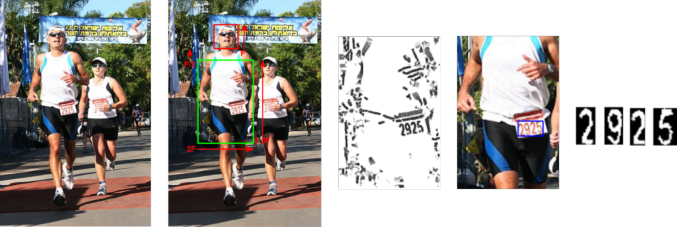
\includegraphics[width=\textwidth]{images/background/benami2012_pipeline}
  \caption[Text recognition pipelines dependent on heuristics]{The \gls{rbn} recognition pipeline by \citet{Benami:2012jf}. \textit{From left to right:} Input image; face detection results in red and the estimated \gls{rbn} region hypothesis in green; \gls{swt} of the hypothesis region; tag region detection in blue; tag region after digit processing.}
  \label{fig:background:recognition:benami2012_pipeline}
\end{figure}

\vspace*{\fill}

\begin{figure}[p]
  \centering
  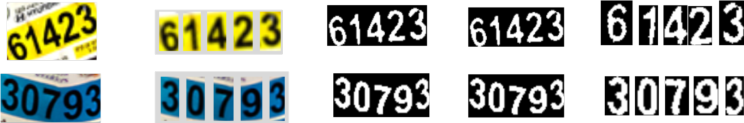
\includegraphics[width=\textwidth]{images/background/benami2012_cctags}
  \caption[Character processing for feeding an OCR engine]{Character processing in \citep{Benami:2012jf}. \textit{From left to right:} A detected tag; separation via \gls{swt} \gls{cc} analysis; binarised characters; \gls{cc} analysis and filtering; separation and alignment.}
  \label{fig:background:recognition:benami2012_cctags}
\end{figure}

\begin{figure}[p]
  \centering
  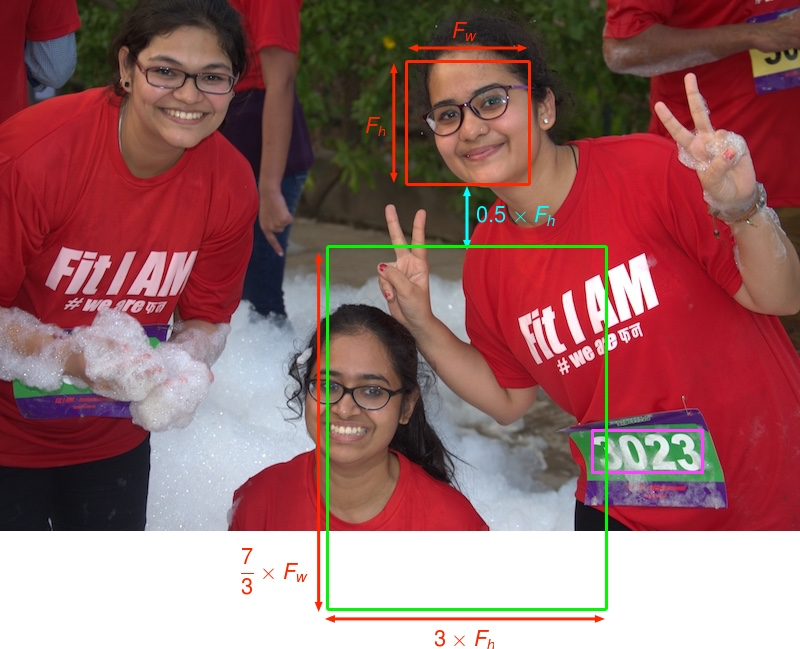
\includegraphics[width=\textwidth]{images/background/benami2012_missed}
  \caption[Drawbacks of heuristic-driven approaches for RBN detection]{Cases where false negatives occur with the heuristic-based approach proposed in \citep{Benami:2012jf}. The expected \gls{rbn} region (shown in magenta) is missed as the subject is leaning in the photo. Face detection in this photo uses the same OpenCV implementation \citep{Lienhart:2002uo} that was used in the study.}
  \label{fig:background:recognition:benami2012_missed}
\end{figure}

\clearpage